%%%%%%%%%%%%%%%%%%%%%%%%%%%%%%%%%%%%%%%%%%%%%%%%%%%%%%%%%%%%%%%%%%%%%%%%%%%
%
% Plantilla para un artículo en LaTeX en doble columna.
%
%%%%%%%%%%%%%%%%%%%%%%%%%%%%%%%%%%%%%%%%%%%%%%%%%%%%%%%%%%%%%%%%%%%%%%%%%%
% !TeX spellcheck = es_ANY
%\documentclass[11pt,twocolumn]{article} %doble columna
%\documentclass[11pt]{article}

\documentclass[12pt,journal, onecolumn]{IEEEtran}
\IEEEoverridecommandlockouts
% The preceding line is only needed to identify funding in the first footnote. If that is unneeded, please comment it out.

\usepackage{url}
\usepackage[utf8]{inputenc}
\usepackage[english]{babel}
\usepackage{fullpage}
\usepackage{graphicx}
\usepackage{array}

\usepackage{subcaption} % subfigures

% Paquetes de la AMS:
\usepackage{amsmath, amsthm, amsfonts, amssymb}

\usepackage{mathtools}

% Atajos.
% Se pueden definir comandos nuevos para acortar cosas que se usan
% frecuentemente. Como ejemplo, aquí se definen la R y la Z dobles que
% suelen representar a los conjuntos de números reales y enteros.
%--------------------------------------------------------------------------

\def\RR{\mathbb{R}}
\def\ZZ{\mathbb{Z}}

% De la misma forma se pueden definir comandos con argumentos. Por
% ejemplo, aquí definimos un comando para escribir el valor absoluto
% de algo más fácilmente.
%--------------------------------------------------------------------------
\newcommand{\abs}[1]{\left\vert#1\right\vert}


%--------------------------------------------------------------------------
\title{Identification of rice genes which respond to saline stress from co-expression network analysis}
\author{Camila Riccio Rengifo\\
  \small Pontificia Universidad Javeriana Cali\\
}

\begin{document}

\maketitle


\section*{Introduction}
Abiotic stresses are the key factors which negatively influence plant development and productivity. They are the main cause of extensive agricultural production losses worldwide. One of the most devastating abiotic stresses, causing reduction in the cultivable land, crop quality and productivity is soil salinity. It has been estimated that 20\% of total cultivated and 33\% of irrigated agricultural lands worldwide are already affected by high salinity. Due to the human activities and natural causes, salinized areas are gradually increasing every year and are expected to reach 50\% by the end of year 2050~\cite{shrivastava2015soil}. Salinity effects are the result of elaborated interactions among morphological, physiological, and biochemical processes. Those processes are regulated by multiple genes and determine the salt tolerance or susceptibility of the crop~\cite{reddy2017salt}. Thus, identifying this group of stress responsive genes may lead to crop improvement in salt tolerance, which is known as a complex quantitative trait. Find this target genes is a complex task, because the function of many genes are still not understood and many novel non-coding genes have been discovered. Particularly rice (\textit{Oryza sativa}), the major food source around the world, is highly sensitive to salt stress~\cite{chang2019morphological}. Therefore, identification of target genes in rice may allow biologist use them as a genetic resource to develop new cultivars with resistance to salinity.\\

We propose a methodology to identify stress responsive genes to salt conditions in rice. The methodology is based on Weighted Gene Co-expression Network Analysis (WGCNA). This is considered an effective and accurate bioinformatic method, using co-expression networks, that has been widely applied in identifying target genes for disease and cancer fields~\cite{tian2018identifying}. We follow the WGCNA workflow but with a new approach in the module detection step. Our modules are detected using the Hierarchical Link Clustering (HLC) technique~\cite{ahn2010link} that allows the recognition of overlapping communities, which may have more biological meaning given the overlapping regulatory domains of systems that generate co-expression~\cite{gaiteri2014beyond}. We conduct a systematic study with a large set of rice data using the proposed methodology. RNA-seq data was accessed through GEO database~\cite{GEOAcces90:online} (Accession number GSE98455), corresponding to $57845$ gene expression profiles of shoot tissues measured for both control and salt condition in $92$ accessions of the Rice Diversity Panel 1. As the analysis result, 6 modules are detected as relevant in the response to salt stress in rice: 3 modules of 3 genes each one associated with shoot K content, 2 modules of 3 genes associated with  shoot biomass, and 1 module of 4 genes associated with root biomass. These genes may act as potential targets for the improvement of salinity tolerance in rice cultivars. From those 19 genes, all but 3 genes (associated with $K$ content), were also identified as deferentially expressed (with a log fold change value greater than $2$) for at least one of the 92 accessions, suggesting that those genes are strong candidates as stress responsive genes. Only 2 of the 16 diferentially expressed genes, both from the module related with shoot biomass, are named and have an associated protein product: Spermidine hydroxycinnamoyltransferase 2 (SHT2) and Lipoxygenase. In other words, further studies are needed to elucidate the detailed biological function of the remaining 14 genes that have not been named so far,  which may have a potential relevance in stress responsive mechanisms to salt conditions in rice.\\

With the development of high-throughput technologies, including microarrays and RNA sequencing (RNA-seq), genome-wide gene expression can be studied under different environmental stimuli (e.g. salt stress). Our methodology uses this kind of transcriptomic data measured for two different conditions (control and stress). After a process of normalization and filtering of the raw data, a differential expression profile of the genes is built calculating the log fold change (LFC) from control to stress condition. The LFC matrix will be the input for the co-expression network construction trough the WGCNA method. A similarity matrix is calculated using the absolute value of Pearson's correlation coefficient between pairs of genes. Then, the similarity matrix is forced to be a scale-free network, finding a beta exponent such that by raising each entry of the matrix to that value, the probability distribution follows a power law. Next, unlike WGCNA, the scale-free network is used to detect overlapping rather than non-overlapping communities, using the HLC technique. We also implement a LASSO regression~\cite{tibshirani1996regression} to select the most significant modules associated with rice phenotypical responses to salt stress. Finally, for the genes found, we look for previous evidence of important biological implications in tolerance to salt stress. That is, the genes deferentially expressed within the selected modules are enriched with gene ontology annotations from QuikGO database~\cite{binns2009quickgo} and their interaction networks reported in STRING database~\cite{szklarczyk2016string} are reviewed.\\

The proposed methodology is modular, since other module detection and selection techniques could be used, instead HLC and LASSO respectively. The advantage of using HLC as clustering method is its ability to detect overlapping modules, since biological components are involved in multiple functions and therefore biological communities tend to be highly overlapping. On the other hand, LASSO is a regularized regression technique widely used in variable selection, thanks to its ability to obtain zero regression coefficients for the less relevant variables~\cite{desboulets2018review}. Additionally, LASSO is especially useful in problems where the number of variables is much larger than the number of samples, which is our case having more than 5000 modules (variables) and 92 accession (samples). The combinations of these techniques would allow finding target genes for future biological studies that evaluate their potential as genes that respond to salt stress in rice. Furthermore, this study can be extended to other stresses and even to other crops.\\

\section{Preliminaries}

\subsection{Co-expression network}
A network is an undirected graph $G=(V,E)$ where ${V=\{v_1,v_2,\ldots,v_{n}\}}$ is a set of \textit{vertices} or \textit{nodes} and ${E=\{e_1,e_2,\ldots,e_q\}}$ is a set of \textit{edges} or \textit{links} that connect vertices. In a gene co-expression network, each node corresponds to a gene. A pair of genes is connected if they show similar differential expression patterns. A simple and unweighted network can be represented by an adjacency matrix $A \in \{0,1\}^{n \times n}$ that is symmetric  with a positive one in the positions $(v_i,v_j)$ and $(v_j,v_i)$ whenever there is an edge connecting vertices $v_i$ and $v_j$, and zeros elsewhere. Co-expression networks are of biological interest because the co-expressed genes are usually controlled by the same transcriptional regulatory pathway, functionally related or members of the same pathway or metabolic complex.\\


\subsection{Hierarchical Link Clustering}

The Hierarchical Link Clustering (HLC) algorithm was proposed by Ahn et al.~\cite{ahn2010link}. The HLC approach represents communities as groups of links (rather than nodes), each node inherits all memberships of its links and can thus belong to multiple, overlapping communities. The algorithm maps links to nodes and connects them if a pair of links shares a node. The similarity between two links $e_{ik}$ and $e_{jk}$ is computed using the Jaccard index 
\begin{equation}
\label{eq:jaccard}
S(e_{ik},e_{jk}) = \frac{\vert n(i) \cap n(j) \vert}{\vert n(i) \cup n(j) \vert},
\end{equation}
where $n(i)$ denotes the set corresponding to node $i$ and its neighbors. The algorithm uses single-linkage hierarchical clustering to build a dendrogram in which each leaf is a link from the original network and branches represent link communities. Hierarchical clustering algorithms repeatedly merge groups until all elements are members of a single cluster.\\

For the purpose of finding meaningful communities it is crucial to know where to partition the dendrogram. In this case, the most relevant communities are established at the maximal partition density $D$, a function  based on link density inside communities measuring the quality of a link partition. The partition density has a single global maximum along the dendrogram in almost all cases, because the value is the average density at the top of the dendrogram (a single giant community with every link and node) and it is very small at the bottom of the dendrogram (most communities consists of a single link). It is the case that $D = 1$ when every community is a fully connected clique and $D = 0$ when each community is a tree. If a community is less dense than a tree (when the community subgraph has  disconnected components), then that community will give a negative contribution to $D $, which can take values less than zero.The minimum density inside a community is $-2/3$,  given by one community of two disconnected edges. Since $D$ is the average of the intra-community density, there is a lower bound of $D=-2/3$. Computing $D$ at each level of the link dendrogram can help the purpose of picking the best level to cut (although meaningful structure could exist above or below the threshold). The output of the process is a set of node clusters, where each node can participate in multiple communities.\\

\subsection{Least Absolute Shrinkage Selector Operator}
The Least Absolute Shrinkage Selector Operator (LASSO) is a regularized linear regression technique. It combines a regression model, with a procedure of contraction of some parameters towards zero and selection of variables, imposing a restriction or a penalty on the regression coefficients. In other words, Lasso solves the least squares problem with restriction on the $ L_1$-norm of the coefficient vector. It can be especially useful to solve problems where the number of variables (e.g., genes) $ n $ is much greater than the number of samples $ m $ (i.e., $ n \gg m $).\\

Consider a dataset consisting of $m$ samples, each of which consists of $n$ covariates and a single outcome. Let $y_i$ be the outcome and $x_i := (x_1,...,x_n)$ be the covariate vector for the $i-th$ sample. Then, the objective of LASSO is to solve

\begin{equation}
\min \left\lbrace\sum_{i=1}^{m}{\left( y_i-\sum_{j=1}^n{\beta_j x_{ij}}\right)^2} \right\rbrace , \textrm{subject to} \sum_{j=1}^n\abs{\beta_j}\leq s
\end{equation}

Or, equivalently, in the so-called Lagrangian form, it minimizes

\begin{equation}
\sum_{i=1}^{p}{\left( y_i-\sum_{j=1}^n{\beta_j x_{ij}}\right)^2} + \lambda \sum_{j=1}^n\abs{\beta_j}
\end{equation}

where $s$ is the regularization penalty and $\lambda \geq 0$ is the corresponding Lagrange multiplier.\\

%LASSO produces parameter estimation and simultaneous variable selection for increasing values of $ \lambda $.

%if $ \lambda = 0 $ the estimator corresponds to the ordinary least squares estimator.

Since the $\lambda$ value determines the degree of penalty, the accuracy of the model depends on its choice. Cross-validation is often used to select the regularization parameter, choosing the one that minimizes the mean-squared error.\\

\section{Methodology}

The proposed methodology uses RNA-seq read counts, representing gene expression levels, as input data. More precisely, it uses $n_0$ gene expression profiles of an organism, measured for $m$ different genotypes under control and treatment conditions, and $r$ biological replicates. This raw data is represented as a matrix $D_0 \in {\mathbb{N}_0}^{n_0 \times 2mr}$. In order to discover key genes and their interaction with phenotypes related to treatment tolerance, the approach also requires a set of $p$ phenotypic traits, measured for the $m$ genotypes. The phenotypic data is seen as a matrix $P \in \mathbb{R}^{2m \times p}$ containing two phenotypic values per genotype, one under control condition and the second one under treatment condition. The whole methodology can be followed in the flow chart of Figure~\ref{fig:flow_chart}.\\

% flow chart
\begin{figure}[]
  \centering
    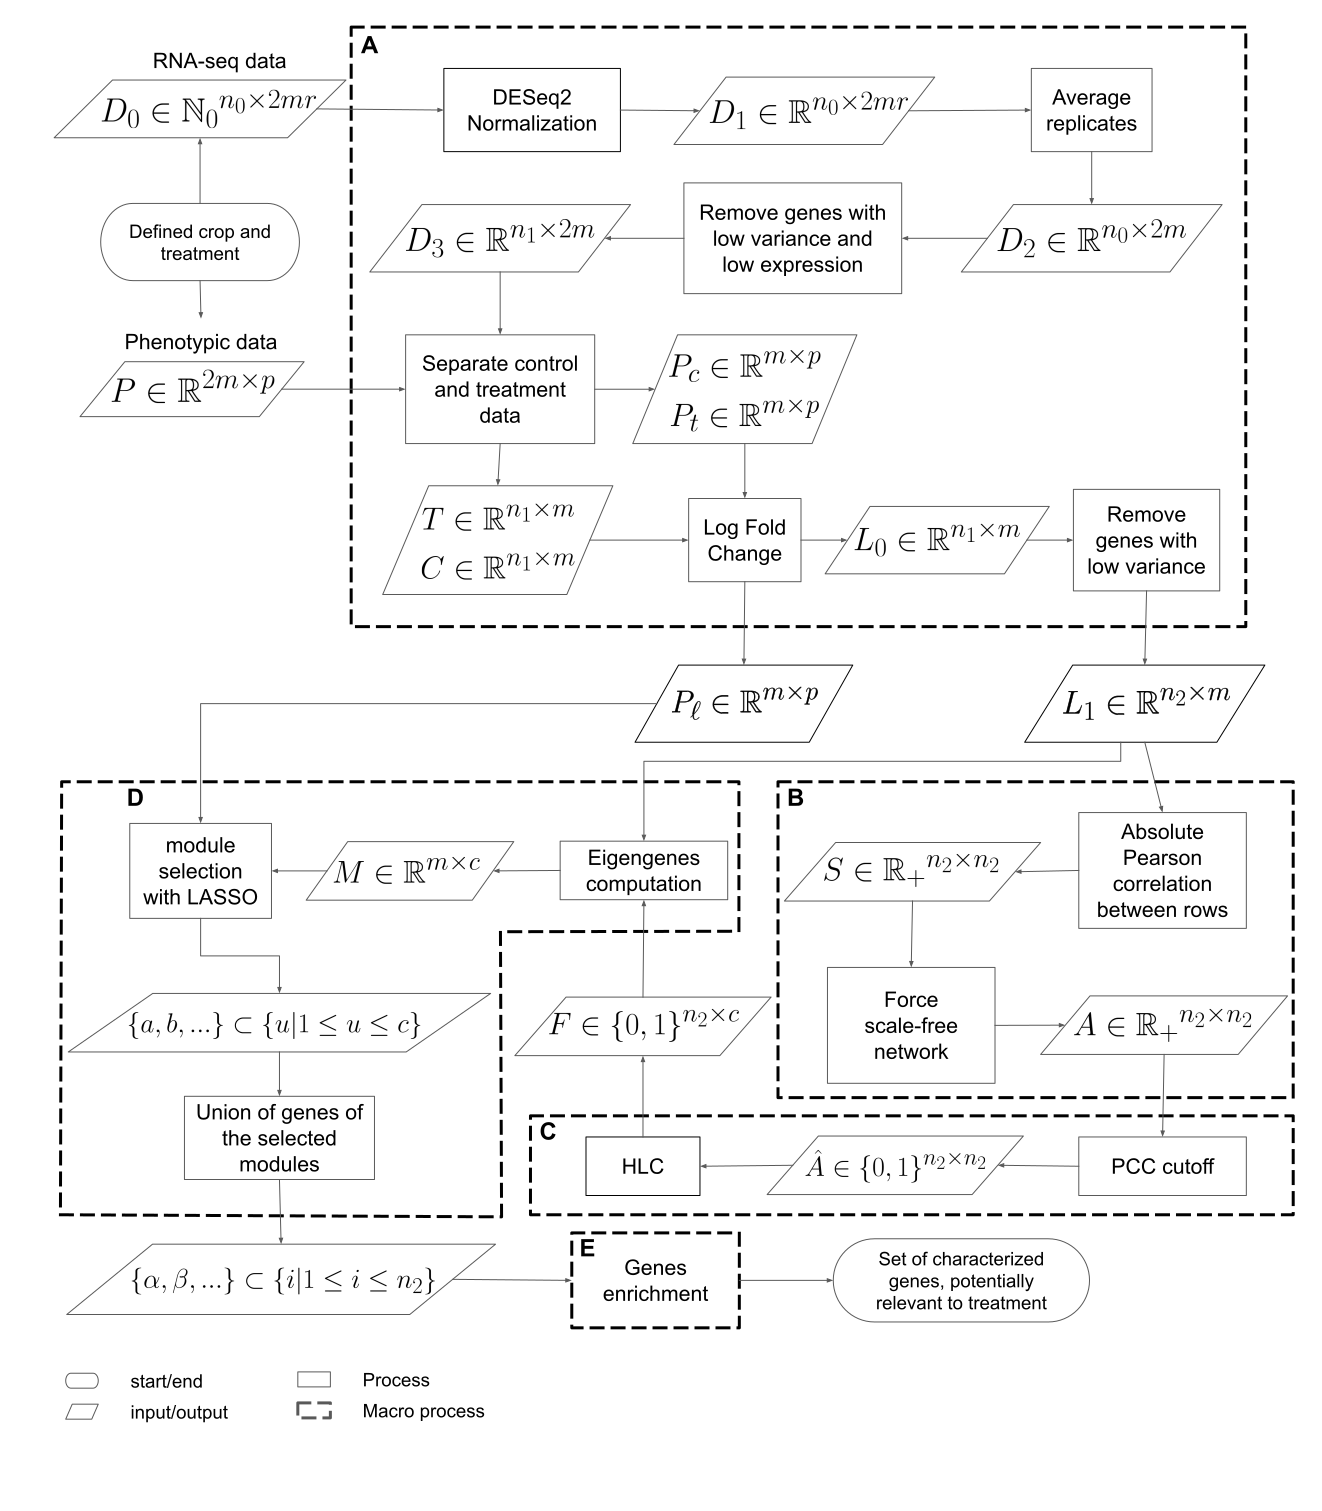
\includegraphics[clip,width=1\textwidth]{Figures/flow_chart.pdf}
  \caption{Proposed methodology flow chart, showing the five macro-processes: \textbf{A}.~Data pre-processing, \textbf{B}.~Co-expression network contruction, \textbf{C}.~Co-expression module identification, \textbf{D}.~Modules association to phenotypic traits, and \textbf{E}.~Genes enrichment.}
  \label{fig:flow_chart}
\end{figure}

\subsection{Data pre-processing}

The RNA-seq data cannot be directly interpreted. Therefore, a normalization process is applied to deal with the problem of some biases affecting the quantification results. In order to correct library size and RNA composition bias, the suggested normalization technique is DESeq2 \cite{love2014moderated}. The normalized data is represented as a matrix $D_1 \in \mathbb{R}^{n_0 \times 2mr}$. The biological replicates of each genotype are averaged and the resulting data is represented as a matrix $D_2 \in \mathbb{R}^{n_0 \times 2m}$. Next, the genes exhibiting low variance or low expression are removed from $D_2$, thus identifying a subset of size $n_1 \leq n_0$ of the original genes. The control and treatment data is separated into the matrices $C\in \mathbb{R}^{n_1 \times m}$ and $T\in \mathbb{R}^{n_1 \times m}$, respectively. The matrix entries $c_{ij}$ in $C$ and $t_{ij}$ in $T$ represent, respectively, the normalized expression level of gene $i$ in accession $j$. Control and treatment data is also separated from phenotypic data $P$, obtaining the $P_c$ and $P_t$ matrices, of dimensions $m \times p$.\\

%From the normalized data $D_1 \in \mathbb{R}^{n_0 \times 2mr}$, average the biological replicates of each genotype, so that the data matrix becomes $D_2 \in \mathbb{R}^{n_0 \times 2m}$. Next, remove genes exhibiting low variance or low expression, getting a new number of $n_1 \leq n_0$ genes. Separate control and treatment data into two matrices $C\in \mathbb{R}^{n_1 \times m}$ and $T\in \mathbb{R}^{n_1 \times m}$, respectively. Each matrix entry, $c_{ij}$ for control and $t_{ij}$ for treatment, represent the normalized expression level of gene $i$ in accession $j$.\\

At this point, the changes in expression levels and phenotypic values, between control and treatment conditions, are measured in terms of logarithmic ratios. In the case of expression levels, the log ratios are represented in a matrix $L_0 \in \mathbb{R}^{n_1 \times m}$, known as the Log Fold Change matrix, where $\ell_{ij}=\log_2 (t_{ij}/c_{ij})$. Similarly, the log ratios of the phenotypic data are computed and represented in a matrix $P_\ell \in \mathbb{R}^{m \times p}$.\\

The final step of the data pre-processing is to filter $L_0$ by removing rows (e.g., genes) with low variance in the differential expression patterns, getting a new matrix $L_1$ of dimensions $n_2 \times m$, with $n_2 \leq n_1$.\\

%Now, compile the control and treatment data by measuring the changes in expression levels in terms of logarithmic ratios. Matrix $L_0 \in \mathbb{R}^{n_1 \times m}$, known as the Log Fold Change matrix, is computed by setting $\ell_{ij}=\log_2 (t_{ij}/c_{ij})$. Repeat this process on the phenotypic data separating the control and treatment data into matrices $P_c$ and $P_t$ of dimensions $m \times p$. Calculate the corresponding logarithmic ratios, obtaining the matrix $P_\ell \in \mathbb{R}^{m \times p}$. Finally, filter $L_0$ matrix by removing rows (genes) with low variance in the differential expression patterns, getting a new matrix $L_1$ of dimensions $n_2 \times m$, with $n_2 \leq n_1$.\\

\subsection{Co-expression network construction}

The Log fold change matrix $L_1$ is used to build the co-expression network following the first two steps of the WGCNA methodology~\cite{langfelder2008wgcna}. First, the level of concordance between gene differential expression profiles across samples is measured. To this end, the absolute value of the Pearson correlation coefficient is used as the similarity measure between genes and the resulting values are stored in the similarity matrix $S\in \mathbb{R_{+}}^{n_2 \times n_2}$.\\

And second, the matrix $S$ is transformed into and adjacency matrix $A \in \mathbb{R_+}^{n_2\times n_2}$ where each entry $a_{ij} = (s_{ij})^\beta $ encodes the connection strength between each pair of genes. In other words, the elements of the adjacency matrix are the similarity values up to the power $\beta > 1$ so the degree distribution will fit a scale-free network. This kind of networks contain many nodes with very few connections and a small number of hubs with high connections. In a strict scale-free network the logarithm of $P(k)$ (the probability of a node to have degree $k$) is approximately inversely proportional to the logarithm of $k$ (the degree of a node). So the parameter $\beta$ is chosen as the smallest value of $\beta$ such that the $R^2$ of the linear regression between $log_{10}(p(k))$ and $log_{10}(k)$ is close to $1$ (e.g. $R^2 > 0.85$). \\

%Then, transform $S$ into an adjacency matrix $A \in \mathbb{R_+}^{n_2\times n_2}$ where each entry $a_{ij} = (s_{ij})^\beta $ encodes the connection strength between each pair of genes. In other words, the elements of the adjacency matrix are the similarity values up to the power $\beta > 1$ so the degree distribution will fit a scale-free network. This kind of networks contain many nodes with very few connections and a small number of hubs with high connections. In a strict scale-free network the logarithm of $P(k)$ (the probability of a node to have degree $k$) is approximately inversely proportional to the logarithm of $k$ (the degree of a node). So the parameter $\beta$ is chosen as the smallest value of $\beta$ such that the $R^2$ of the linear regression between $log_{10}(p(k))$ and $log_{10}(k)$ is close to $1$ (e.g. $R^2 > 0.85$). \\


\subsection{Co-expression module identification}

Next step in the methodology is to study the co-expression network structure and dynamics identifying communities also called modules. The idea is to cluster genes with similar differential expression change patterns. Membership in these modules may overlap in biological contexts, where modules may be related to specific molecular, cellular or tissue functions and the biological components (i.e. genes) are involved in multiple functions. Thus, unlike WGCNA, the adjacency matrix $A$, is used to detect overlapping (rather than non-overlapping) communities, using the Hierarchical Link Clustering (HLC) algorithm proposed in~\cite{ahn2010link}.\\

%HLC approach reinvent communities as groups of links rather than nodes, each node inherits all memberships of its links and can thus belong to multiple overlapping communities. The algorithm maps links to nodes and connects them if a pair of links shares a node. The similarity between links is computed using the Jaccard index. With this similarity, they use single-linkage hierarchical clustering to build a dendrogram where each leaf is a link from the original network and branches represent link communities. Finally, the most relevant communities are established at the maximal partition density, a function  based on link density inside communities.\\

As a previous step, matrix $A$ has to be modified, in order to apply the clustering algorithm, transforming it into an unweighted network $\hat{A} \in \{0,1\}^{n_2 \times n_2}$. To this end, the Pearson Correlation Coefficient (PCC) cutoff is determined using the approach described by~\cite{aoki2007approaches} based on density of the network combined with decreasing number of nodes and edges with higher PCC values. Above the cutoff, the entries of matrix $A$ become $1$, and below the cutoff $A$ values becomes zero.\\

%To determine the Pearson Correlation Coefficient (PCC) cutoff for finding biologically relevant co-expressed modules, we use the approach described by~\cite{aoki2007approaches} based on density of the network combined with decreasing number of nodes and edges with higher PCC values. Above the cutoff, the entries of matrix $A$ become $1$ and when the value is below the threshold it becomes zero.\\

Now, the HLC algorithm can be applied. It organizes the $n_2$ genes of matrix $\hat{A}$ into $c$ communities, where each gene can belong to one, multiple, or no community. This information is represented as an affiliation matrix $F \in \{0,1\}^{n_2 \times c}$, where $f_{iu} = 1$ if node $i$ is member of cluster $u$.\\ 

\subsection{Modules association to phenotypic traits}

To identify the most relevant groups (modules) of genes, associated with the phenotypic response to a specific treatment in an organism, the proposed methodology uses a LASSO based approach. Each module is represented by a eigengene, which is defined as the first principal component of such module. A eigengene can be thought of as an average differential expression profile for each community and is computed from the Log Fold Change Matrix $L_1$ and the affiliation matrix $F$. Given a module $u$, the affiliation matrix is used to identify the genes belonging to $u$ and then the corresponding rows of the matrix $L_1$ are selected to compute the first principal component of $u$. Each principal component becomes a column of the matrix $M \in \mathbb{R}^{m \times c}$.\\   

% the Log Fold Change matrix rows corresponding to the genes belonging to a specific module. \\

These profiles are then associated with each phenotypic trait using the least absolute shrinkage and selection operator (LASSO).
%LASSO combines a regression model with a procedure of contraction of some parameters towards zero, imposing a restriction or a penalty on the regression coefficients. 
This technique allows selection of the most relevant variables. In our context, the eigenges (the columns of $M$) act as regressor variables and each phenotypic trait (each column of $P_\ell$) is used as an outcome variable at a time.\\

The output after applying LASSO is a set of modules for each phenotypic trait. The union of genes belonging to the selected modules are the target genes for downstream analysis.\\

\subsection{Genes enrichment}

The objective of this part of the analysis is to characterize the genes found with complementary information, helping to elucidate their possible behavior and role in the response to the studied treatment.\\

A simple analysis to made with the selected genes, using the previous calculations, is to identify the differentially expressed ones. That is, identify genes showing an absolute value of the log fold change greater than 2 ($|\ell_{ij}|\geq 2$) for at least one sample. This represents genes whose level of expression is quadrupled (up or down) from control to treatment condition, suggesting that those genes are strong candidates as treatment responsive genes.\\

A widley used approach in this step is to perform a functional category enrichment, searching for the Gene Ontology (GO) annotations from databases like QuikGO~\cite{binns2009quickgo}. This annotations can provide evidence of biological implications of the target genes in the treatment-tolerance mechanisms.\\

Addicionally, QuickG0 can be used to identify genes with reported protein products, which can be used to perform another relevant analysis reviewing their reported protein-protein interaction networks using the STRING database~\cite{szklarczyk2016string}. The interactions include direct (physical) and indirect (functional) associations; they stem from computational prediction, from knowledge transfer between organisms, and from interactions aggregated from other (primary) databases. This information elucidates how the selected genes are involved in functional pathways that can be related with the treatment of interest.\\

% Otras caracteristicas pueden buscarse en otras bases de datos o hacer una busqueda más exahustiva en articulos de estudios previos sobre estos genes.

\section{Case study}
The RNA-seq data was obtained from GEO database \cite{GEOAcces90:online} (accession number GSE98455). This data corresponds to $n_0=57845$ gene expression profiles of shoot tissues measured for both control and salt condition in $m=92$ accessions of the Rice Diversity Panel 1, with $r=2$ biological replicates. A total of $p=3 $ phenotypic traits are used: shoot $K^+$ content, root biomass and shoot biomass. These traits were measured for the same $92$ genotypes, under  control and salt stress conditions, and can be found in the supplementary information of~\cite{campbell2017allelic}.\\

\subsection{Data pre-processing}
DESeq2 normalization was applied to the raw data and the biological replicates were averaged. Genes exhibiting low variance were identified as those with ratio of upper quantile to lower quantile smaller than $1.5$, and were removed from the normalized data. Genes with low expression, corresponding to those having more than $80\%$ samples with values smaller than $10$, were also removed. A total of $n_1 = 8928$ genes were kept after this filtering process.\\

From the Log Fold Change matrix $L_0$, genes whose difference between upper quantile and lower quantile was greater than $0.25$, were removed. Therefore, the resulting matrix $L_1$ contains the log ratios of $n_2 = 8928$ genes. The logarithmic ratios of the phenotipic data, for the $92$ accessions and the $3$ traits, was also computed.\\   

\subsection{Co-expression network construction}
The Log Fold Change matrix $L_1$ is used to compute the corresponding similarity matrix. 
For this network, it was observed that $\beta=3$ is the smallest integer such that the $R^2 \geq 0.8 $. Figure~\ref{fig:beta} shows the degree distribution of the similarity matrix (left) and the degree distribution of the adjacency matrix (right), which is the degree distribution of a scale-free network with $R^2 = 0.8$ with $\beta = 3$.

%scale-free beta 1 y 3
\begin{figure}[h]
  \centering
    \includegraphics[clip,width=0.8\textwidth]{Figures/pick_beta.png}
  \caption{Degree distributions}
  \label{fig:beta}
\end{figure}

The resulting adjacency matrix $A$ represents a complete graph $G=(V,E)$, with $|V| = 8928$ genes and $|E| = 39850128$ edges. The cutoff value was set to $0.2$, thus keeping only the connections above this threshold and removing the isolated nodes. The resulting adjacency matrix $\hat{A}$ has $n_3 = 5810$ genes and accounts for $16875145$ edges.\\

%The current network represented by the adjacency matrix $A$, corresponds to a complete and weighted network of $8928$ genes (nodes) and $39850128$ edges. For computational reasons, this network was transformed into an unweighted one $\hat{A}$, keeping only the connections above the cutoff value of $0.2$. The resulting unweighted network has a total of $5810$ nodes and $16875145$ edges. 

\subsection{Co-expression module identification}
After applying the HLC algorithm, a total of $4131$ genes were distributed in $c = 5143$ overlapping modules of $3$ or more genes. Figure~\ref{fig:overlap} shows a histogram of the overlapping percentage of these genes, measured as the proportion of modules to which each gene belongs. The first bar of the histogram represents the genes with zero overlap, which correspond to $28\%$ of the total genes, the other $72\%$ represents genes belonging to more than one module.

%overlapping percentage
\begin{figure}[h]
  \centering
    \includegraphics[clip,width=0.5\textwidth]{Figures/artificial_modules.png}
  \caption{Overlapping percentage}
  \label{fig:overlap}
\end{figure}


\subsection{Modules association to phenotypic traits}
The phenotypic traits under study are shoot $K^+$ content, root biomass and shoot biomass. Figure \ref{fig:pdata} suggests that there are significant differences in the values of these phenotypic traits between stress and control conditions. This supports the working hypothesis that these three variables represent tolerance-associated traits in rice under salt stress.\\

% boxplots
\begin{figure}[h]
  \centering
    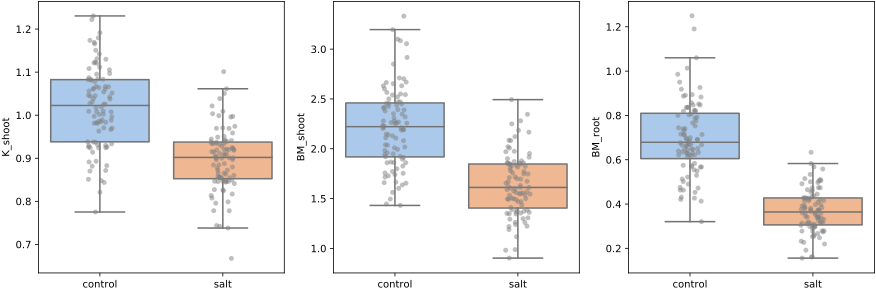
\includegraphics[clip,width=1\textwidth]{Figures/phenotypic_traits.png}
  \caption{Phenotipic traits distribution under control and salt stress}
  \label{fig:pdata}
\end{figure}

Using the affiliation matrix $F$ derived from the HLC output and the Log Fold Change matrix $L_1$, a matrix $M$ is built by computing the egengene for each of the $c = 5143$ modules. The LASSO technique was applied by using each of the phenotypic traits as the outcome variable, one at a time. As shown in Figure~\ref{fig:cross-val} cross-validation was performed for each phenotypical trait in order to select the corresponding regularization parameter $\lambda$ that minimizes the mean-squared error.\\

%we build the matrix $M$ computing the egengene for each of the $c = 5143$ modules. We apply the LASSO technique using each of the phenotypic traits as the outcome variable, one at a time. As shown in Figure~\ref{fig:cross-val} we perform cross-validation for each phenotypical trait, in order to select the corresponding regularization parameter $\lambda$ that minimizes the mean-squared error.\\

\begin{figure}[h]
\centering
   \begin{subfigure}{0.3\linewidth} \centering
     \includegraphics[width=1\textwidth]{Figures/lambda_kshoot_2.png}
     \caption{$K$ shoot, $\lambda = 0.013$}\label{fig:lambda_kshoot}
   \end{subfigure}
   \begin{subfigure}{0.3\linewidth} \centering
     \includegraphics[width=1\textwidth]{Figures/lambda_BMshoot_2.png}
     \caption{Shoot biomass, $\lambda = 0.025$}\label{fig:lambda_BMshoot}
   \end{subfigure}
   \begin{subfigure}{0.3\linewidth} \centering
     \includegraphics[width=1\textwidth]{Figures/lambda_BMroot.png}
     \caption{Root biomass, $\lambda = 0.035$}\label{fig:lambda_BMroot}
   \end{subfigure}
\caption{Cross-validation of the LASSO regularization parameter $\lambda$, for each phenotypic trait.} \label{fig:cross-val}
\end{figure}

FInally, three LASSO models were adjusted by using the corresponding $\lambda$ and phenotypical data with the egengens of matrix $M$. As result, 6 modules were detected as relevant in the response to salt stress in rice: 3 modules of 3 genes each one associated with shoot $K$ content, 2 modules of 3 genes associated with  shoot biomass, and 1 module of 4 genes associated with root biomass.\\

\subsection{Genes enrichment}
From the $19$ genes selected by LASSO, all but $3$ genes (associated with $K$ content), were also identified as deferentially expressed ($|\ell_{ij}| \geq 2$) for at least one of the $92$ accessions. This suggest that those genes are strong candidates as stress responsive genes to salt conditions in rice.\\

According to the Quickgo database, only $2$ of the $16$ diferentially expressed genes, both from the module related with shoot biomass, are named and have an associated protein product: Spermidine hydroxycinnamoyltransferase 2 (SHT2) and Lipoxygenase. Figure~\ref{fig:3d} shows their corresponding 3D protein structure.

% Figure 3d protein strucures
\begin{figure}[h]
\centering
   \begin{subfigure}{0.49\linewidth} \centering
     \includegraphics[width=0.5\textwidth]{Figures/structure_LOC_Os12g27254.png}
     \caption{Spermidine hydroxycinnamoyltransferase 2}\label{fig:structure_SHT2}
   \end{subfigure}
   \begin{subfigure}{0.49\linewidth} \centering
     \includegraphics[width=0.5\textwidth]{Figures/structure_LOC_Os12g37260.png}
     \caption{Lipoxygenase}\label{fig:structure_Lipoxygenase}
   \end{subfigure}
\caption{3D protein structure of named genes selected by LASSO.} \label{fig:3d}
\end{figure}

Uniprot database~\cite{uniprot2018uniprot} reports, on the one hand, that SHT2 contributes to the natural variation of spermidine-based phenolamides in rice cultivars. On the other hand, is reported that plant lipoxygenase may be involved in a number of diverse aspects of plant physiology including growth and development, pest resistance, and senescence or responses to wounding. This protein is involved in the pathway oxylipin biosynthesis, which is part of Lipid metabolism. Aditionally, previous studies (\cite{gupta2013plant, hou2015persimmon, mittova2002salt, peng2019novel, roychoudhury2011amelioration}) provide evidence of biological implications of sperimidine and lipoxygenase in tolerance to salt stress in other plants or even in rice cultivars. However, further studies are needed to elucidate the detailed biological function of the remaining 14 genes that have not been named so far,  which may have a potential relevance in stress responsive mechanisms to salt conditions in rice.

%We also use the STRING database to visualize the reported interaction networks of the 2 named genes (see Figure X). 

%Figure STRING networks




\section{Discussion}

This manuscript provides a detailed description of a network analysis-based methodology to 
%The methodology described in this manuscript provides network analysis-based approach to
the discovery of key genes responding to a specific treatment in an organism, linking transcriptomic with phenotypic data, and identifying overlaping gene modules.\\

The proposed methodology is inspired by the workflow suggested by the WGCNA methodology~\cite{langfelder2008wgcna}. The main steps are the preprocessing of the gene expression data, the construction of a co-expression network, the detection of modules within the network, relate the modules with external information (e.g. phenotypic data) and an enrichment of the identified key genes. The methodology is structured in a modular way, which allows modifying and exploring different techniques in each of the steps of the process. \\

%The proposed methodology follows the principles of WGCNA. Starts from the level of thousands of genes, identifies biologically interesting gene modules, and identifies key genes in the treatment pathways for further validation. In WGCNA the whole workflow is structured in a modular way. The proposed methodology takes advantage of this property modifying and exploring new techniques inside some processes.\\

The proposed approach is designed to integrate expression data measured under two different conditions (control and treatment), unlike the usually co-expression-based approaches which work with both conditions independently or consider a single condition. For this purpose, an approach similar to that proposed in~\cite{du2019network} is used, where the control and treatment data are compiled in a single matrix using the log fold change measure. Thus, the input to construct the co-expression network is not the expression data but the changes in the expression levels from one condition to the other, allowing to capture the signal of changes caused by the treatment.\\

Another important innovation in the proposed methodology is the module detection technique. The co-expression network is calculated as in WGCNA until the scale-free network is obtained. This network is then used to apply the HLC algorithm, a clustering technique capable of detecting overlapping communities. Several approaches of module detection from gene expression have been proposed and were evaluated in~\cite{saelens2018comprehensive}. Most of them focuses only on disjoint (non-overlapping) communities and the described techniques dealing with overlap are not clustering but biclustering and decomposition methods. It is well known that communities in real networks are overlapping. Thus the approach presented in this work can be seen as a generalization of the previous approaches.\\

%Similar approximations have been proposed in, e.g., \cite{langfelder2008wgcna} and \cite{du2019network}, but they only focus on disjoint (non-overlapping) communities. It is well known that communities in real networks are overlapping, and thus the approach presented in this work can be seen as a generalization of the previous approaches.\\

% La tercera modificación es incluir LASSO como método para relacionar los datos phenotypicos con los transcriptomicos.

The methodology was applied in a case study with rice under salt stress. The results show a group of 14 genes where two of them are related to the response to saline stress according to previous studies, validating the ability of the method to detect this kind of key genes.\\

As future work, other overlapping module detection and selection techniques could be used, instead HLC and LASSO respectively. The combinations of these techniques would allow finding target genes for future biological studies that evaluate their potential as genes that respond to salt stress in rice. Furthermore, this study can be extended to other stresses and even to other crops.\\


\bibliographystyle{acm}
\bibliography{mybibliography}

\end{document}
